% Created 2018-10-17 Mi 17:38
% Intended LaTeX compiler: pdflatex
\documentclass[11pt]{article}
\usepackage[utf8]{inputenc}
\usepackage[T1]{fontenc}
\usepackage{graphicx}
\usepackage{grffile}
\usepackage{longtable}
\usepackage{wrapfig}
\usepackage{rotating}
\usepackage[normalem]{ulem}
\usepackage{amsmath}
\usepackage{textcomp}
\usepackage{amssymb}
\usepackage{capt-of}
\usepackage{hyperref}
\usepackage{float}
\author{Nikolai Weidt}
\date{\today}
\title{Calcback}
\hypersetup{
 pdfauthor={Nikolai Weidt},
 pdftitle={Calcback},
 pdfkeywords={},
 pdfsubject={},
 pdfcreator={Emacs 26.1 (Org mode 9.1.14)}, 
 pdflang={English}}
\begin{document}

\maketitle
\setcounter{tocdepth}{2}
\tableofcontents



\section{What is this?}
\label{sec:org41cfd18}
This is a script to get the complex refractive index \(n = n * ik\) from the ellipsometric parameters \(\Delta\) and \(\Psi\) I got from a simulation.
The result for 300nm SiO\(_{\text{2}}\) should look like this:

\begin{figure}[htbp]
\centering
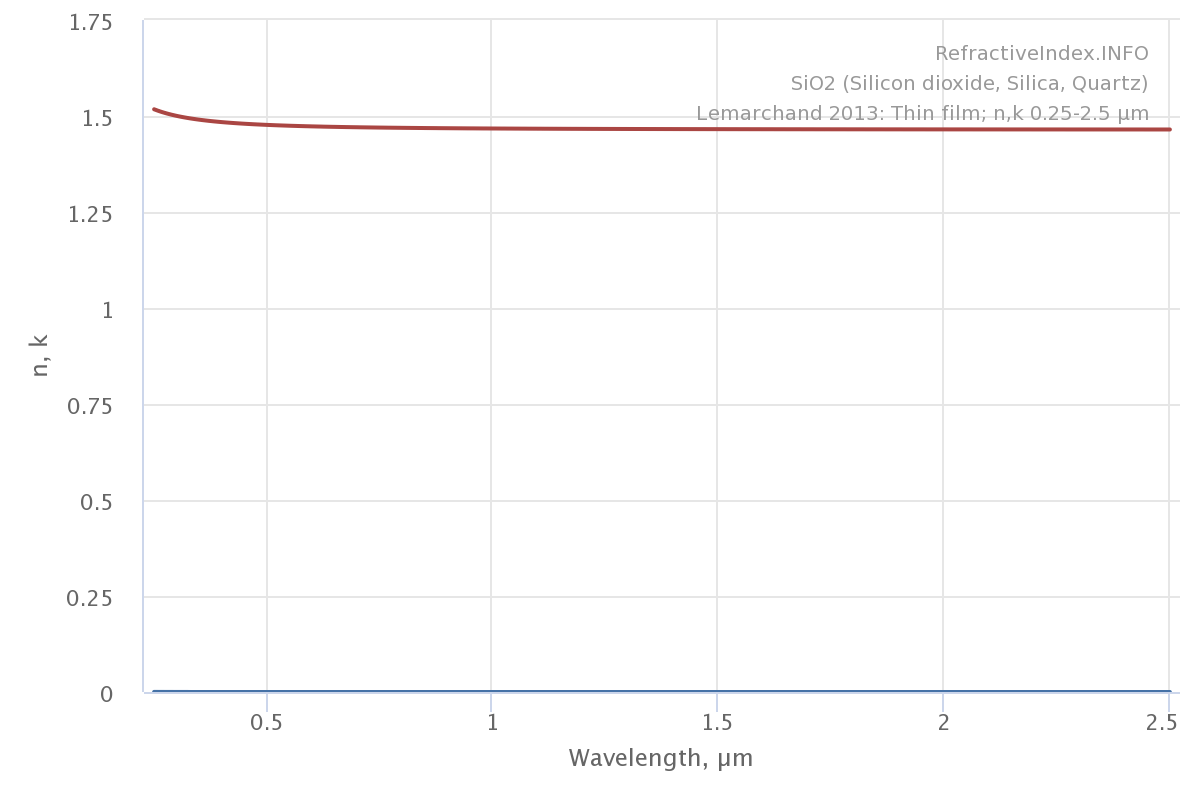
\includegraphics[width=\textwidth]{./RefractiveIndexSiO2.png}
\caption{\label{fig:orga0d4ae7}
Refractive index should look like this}
\end{figure}
\section{List of Todos:}
\label{sec:orgdd2ce71}
\subsection{{\bfseries\sffamily TODO} Write a loop for all wavelengths after it works for one.}
\label{sec:org4253924}

\subsection{{\bfseries\sffamily TODO} Then take even more wavelengths (rows)}
\label{sec:org1a70d49}
\section{Imports:}
\label{sec:org822dd54}
\begin{verbatim}
import numpy as np
import matplotlib
matplotlib.use('Agg')
import matplotlib.pyplot as plt
\end{verbatim}

\section{Defining some variables:}
\label{sec:org1b7bbc9}
Defining some variables for later use:

\begin{verbatim}
CSVFILE = "head300nmSiO2.csv"  # head = only 10 rows of data
phi_i = 70 * np.pi / 180  # converting incident angle from deg (first number) to rad
d_L = 300  # thickness of layer in nm
n_air = 1  # refractive index of air
rerange = 5  # upper limit for real part
imrange = 1  # upper limit for imaginary part
i = 0  # only look at one wavelength (row in csv)
\end{verbatim}

\section{Read .csv-file:}
\label{sec:org9bc78f5}
Read the values into a two dimensional numpy array as [[lambda,Psi,Delta,n\(_{\text{S}}\), k\(_{\text{S}}\)],\ldots{}] (Skip columns 3 and 4)

\begin{verbatim}
csv = np.loadtxt(CSVFILE, usecols=(0,1,2,5,6),  delimiter=",", skiprows=1)
\end{verbatim}

The array looks like this:
\begin{verbatim}
csv
\end{verbatim}

\begin{verbatim}
[[300.          55.2217535   84.37228319   2.6726       3.0375    ]
 [303.          50.11187439  93.3085011    2.7346       3.0381    ]
 [306.          46.35824553  98.43681392   2.7967       3.0368    ]
 [309.          43.50539341 101.18051798   2.8588       3.0334    ]
 [312.          41.29392865 102.19236832   2.9206       3.0279    ]
 [315.          39.48751217 101.93002      2.9822       3.0205    ]
 [318.          37.90308303 100.64846104   3.0435       3.0109    ]
 [321.          36.47640803  98.54577151   3.1042       2.9994    ]
 [324.          35.12615859  95.72242205   3.1644       2.9858    ]]
\end{verbatim}

\section{Calculate \(\rho\)}
\label{sec:org4de4882}
\subsection{Create a matrix containing every possible refractive index (n+ik):}
\label{sec:org80021ca}

Change the last number in the "linspaces" to adjust the resolution.

\begin{verbatim}
lsp_re = np.linspace(1, rerange, 1001)
lsp_im = np.linspace(0.01, imrange, 1001)
re, im = np.meshgrid (lsp_re, lsp_im, copy=False)
n_L = 1j * np.round(im,6) + np.round(re,6)
n_L = n_L.flatten() # create onedimensional array
\end{verbatim}

This gives the following matrix:
\begin{verbatim}
n_L
\end{verbatim}

\begin{verbatim}
[1.   +0.01j 1.004+0.01j 1.008+0.01j ... 4.992+1.j   4.996+1.j
 5.   +1.j  ]
\end{verbatim}

\subsection{Calculate \(\rho\):}
\label{sec:org5d8c938}
\subsubsection{First we define some functions:}
\label{sec:org82e60c1}
\begin{enumerate}
\item Snell's Law to calculate the refractive angles:
\label{sec:org82db8b0}
Phi is the incident angle for the layer, n1 and n2 are refractive indices of first and second medium. Returns the angle of refraction.

\begin{figure}[H]
\centering
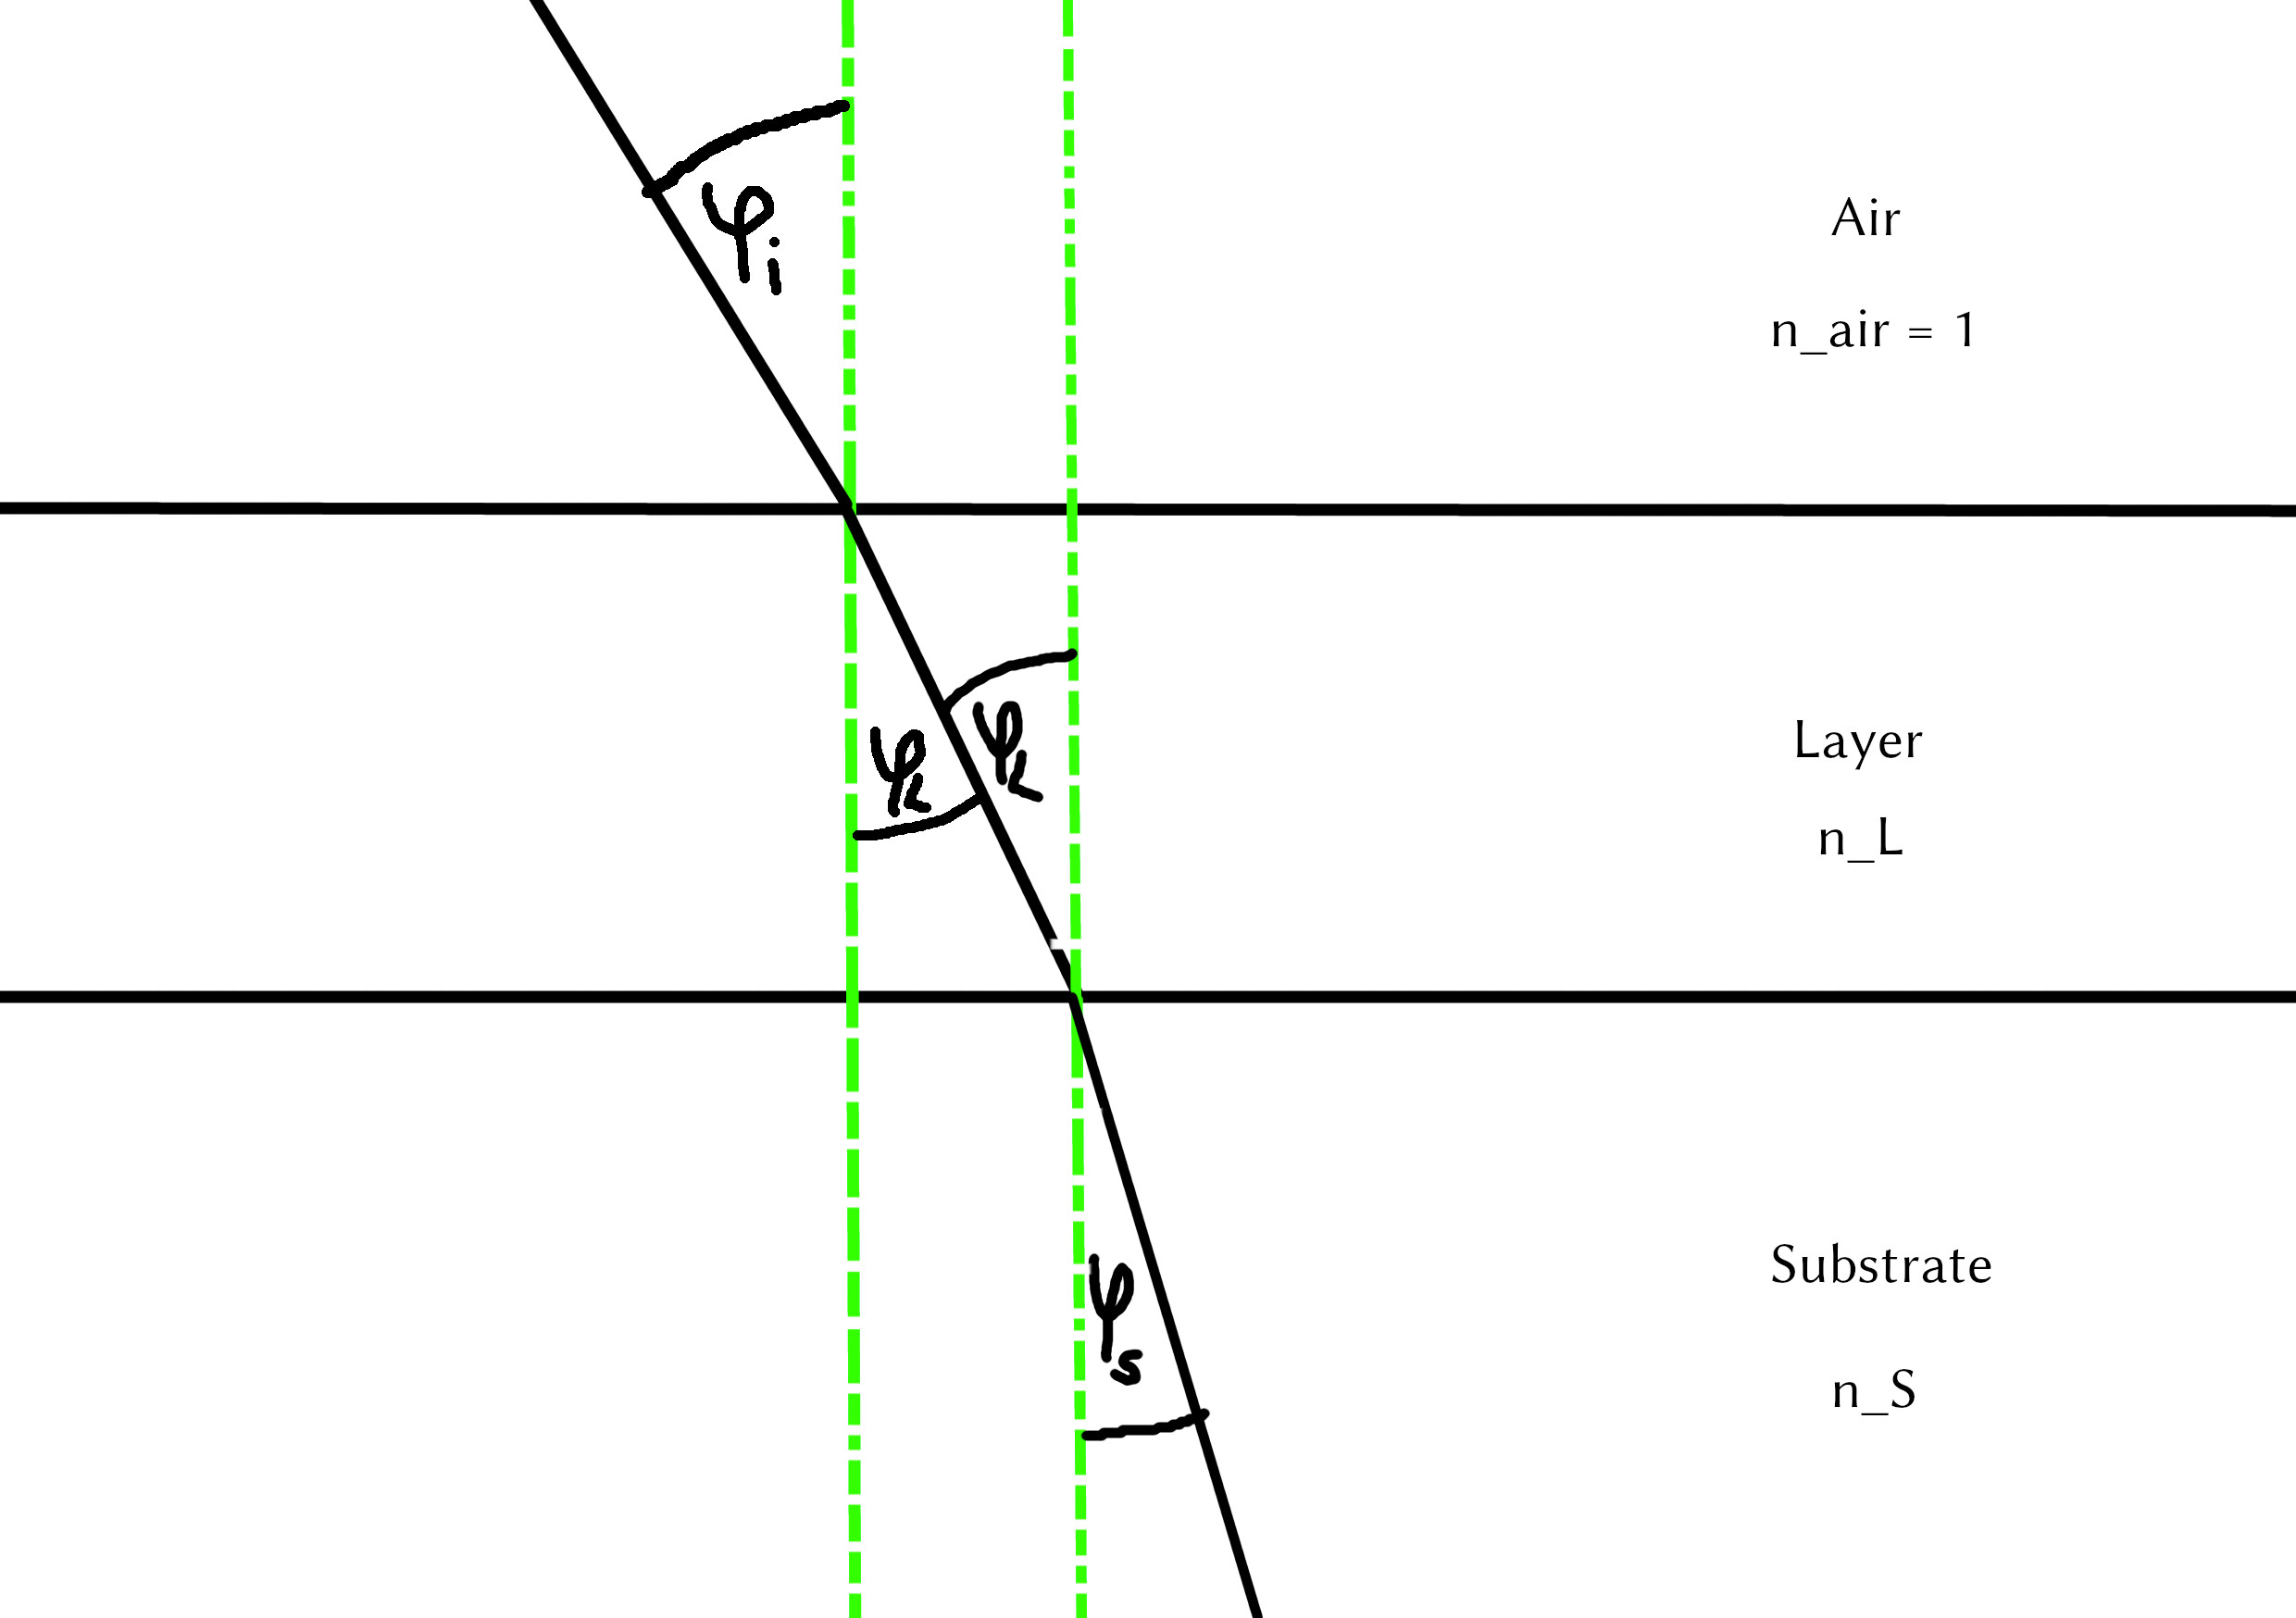
\includegraphics[width=\textwidth]{./snell.jpg}
\caption{\label{fig:org79a5148}
Snell's Law}
\end{figure}
\begin{verbatim}
def snell(phi, n1, n2):
    phi_ref = np.arcsin((np.sin(phi) * n1) / n2)
    return phi_ref
\end{verbatim}


\item Calculate r\(_{\text{p}}\) and r\(_{\text{s}}\) with Fresnel equations:
\label{sec:orgdd5ff0c}
\begin{verbatim}
def fresnel(n1, phi1, n2, phi2):
    """Takes refractive indices and angles of two layers to calculate the amplitude reflection coefficients"""
    rs = (n1 * np.cos(phi1) - n2 * np.cos(phi2)) / (n1 * np.cos(phi1) + n2 * np.cos(phi2))
    rp = (n2 * np.cos(phi1) - n1 * np.cos(phi2)) / (n2 * np.cos(phi1) + n1 * np.cos(phi2))
    return rs, rp
\end{verbatim}


\item Calculate \(\rho\) for the layer with eq. 5.2 in Spectroscopic Ellipsometry \citenum{fujiwara2009spectroscopic}:
\label{sec:org8983924}
\begin{verbatim}
def calc_rho(rs_al, rp_al, rs_ls, rp_ls, d_L, n_L, lambda_vac):
    beta = 2 * np.pi * d_L * n_L * np.cos(phi_L) / lambda_vac
    rp_L = (rp_al + rp_ls * np.exp(-2*1j*beta)) / (1 + rp_al * rp_ls * np.exp(-2 * 1j * beta))
    rs_L = (rs_al + rs_ls * np.exp(-2*1j*beta)) / (1 + rs_al * rs_ls * np.exp(-2 * 1j * beta))
    rho = rp_L / rs_L
    return rho
\end{verbatim}
\end{enumerate}


\subsubsection{Then we call these functions one after another to calculate \(\rho\):}
\label{sec:org4140bbd}
Get refractive index of the substrate (n\(_{\text{S}}\)) and lambda from the csv:
\begin{verbatim}
lambda_vac = csv[i, 0]
n_S = (csv[i, 3] + 1j * csv[i, 4])
\end{verbatim}

Then call the above defined functions
\begin{verbatim}
phi_L = snell(phi_i, n_air, n_L)
phi_S = snell(phi_L, n_L, n_S)
# Fresnel equations:
# air/layer:
rs_al, rp_al = fresnel(n_air, phi_i, n_L, phi_L)
# layer/substrate:
rs_ls, rp_ls = fresnel(n_L, phi_L, n_S, phi_S)

rho_L = calc_rho(rs_al, rp_al, rs_ls, rp_ls, d_L, n_L, lambda_vac)
\end{verbatim}


\subsubsection{Identify the best fitting rho with \(\rho\) = tan(\(\psi\)) * e\(^{\text{i}\Delta}\) :}
\label{sec:org0412a54}

\begin{verbatim}
# psi is in our csv-file at index 1, delta at index 2 at row "i" for lambda
psi = csv[i][1]
delta = csv[i][2]
rho = np.tan(psi) * np.exp(1j * delta)
diff = abs(rho - rho_L)  # magnitude of complex number
idx = np.argmin(diff)  # index of the minimum
minimum = diff[idx]
n = n_L[idx]
print("The layer has the refractive index n_L = ", n)
\end{verbatim}

\begin{verbatim}
The layer has the refractive index n_L =  (4.008+0.15157j)
\end{verbatim}

\section{Plot some things for checking results:}
\label{sec:orga8b9e66}

If we use a high resolution, those plots are not showing much, thats why they are only showing the first 10000 values.
\subsection{Plot real and imaginary part of the created n\(_{\text{L}}\) matrix:}
\label{sec:org7918754}

Real part is blue, imaginary is red.

\begin{verbatim}
fig = plt.figure()
plt.plot(np.real(n_L[:10000]), c='b')
plt.plot(np.imag(n_L[:10000]), c="r")
plt.savefig('n_L.png')
'./n_L.png'

\end{verbatim}

\begin{center}
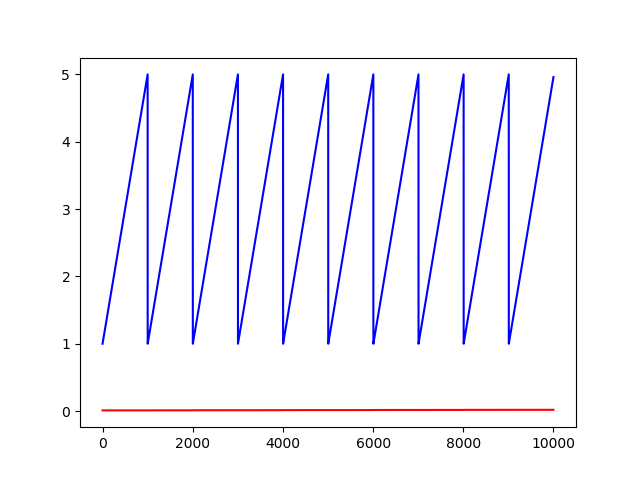
\includegraphics[width=.9\linewidth]{./n_L.png}
\end{center}

\subsection{Plot real and imaginary part of \(\rho_{\text{L}}\)}
\label{sec:orgc9d8cf9}

\begin{verbatim}
fig = plt.figure()
plt.plot(np.real(rho_L), c='b')
plt.plot(np.imag(rho_L), c='r')
plt.savefig('rho_L.png')
"./rho_L.png"
\end{verbatim}

\begin{center}
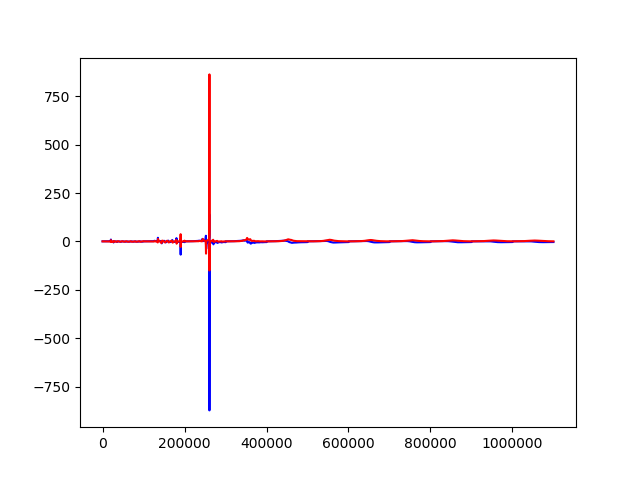
\includegraphics[width=.9\linewidth]{./rho_L.png}
\end{center}

\subsection{Plot of the difference between \(\rho_{\text{L}}\) and the given \(\rho\) and determined minimum:}
\label{sec:org2c6ddbd}

The difference is shown in blue, the red lines show the minimum.

\begin{verbatim}
fig = plt.figure()
plt.axvline(idx, c='r')
plt.axhline(minimum, c='r')
plt.plot(diff[:idx+10000])
plt.savefig('diff.png')
"./diff.png"
\end{verbatim}

\begin{center}
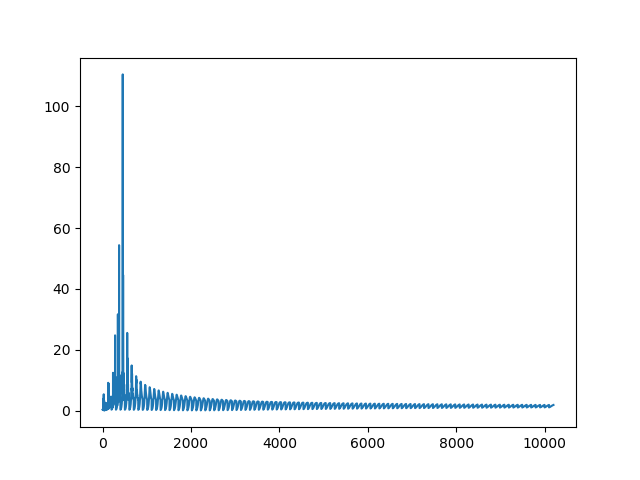
\includegraphics[width=.9\linewidth]{./diff.png}
\end{center}

\subsection{Plot refractive angle phi\(_{\text{L}}\) and n\(_{\text{L}}\):}
\label{sec:orgf4eb4db}

n\(_{\text{L}}\) is shown in green, real part of phi\(_{\text{L}}\) in blue, imaginary in red. 
A relation between these should be visible.

\begin{verbatim}
fig = plt.figure()
plt.plot(np.real(phi_L[:5000]), 'b')
plt.plot(np.imag(phi_L[:5000]), 'r')
plt.plot(np.real(n_L[:5000]), c='g')
plt.savefig('phi_L.png')
"phi_L.png"
\end{verbatim}

\begin{center}
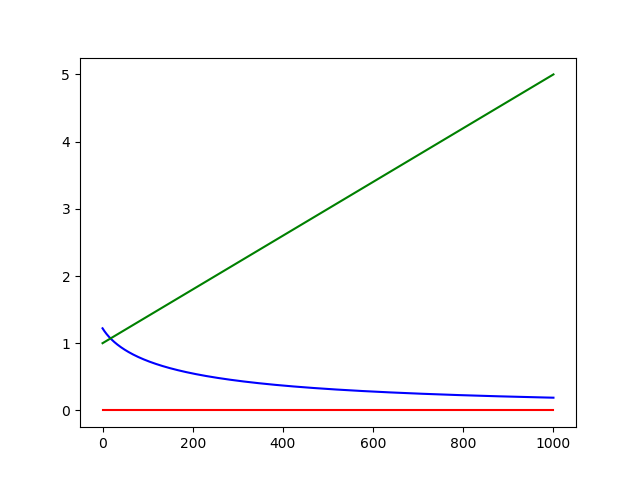
\includegraphics[width=.9\linewidth]{phi_L.png}
\end{center}

\bibliography{forschungspraktikum}
\end{document}